\documentclass[11pt]{article}
\usepackage[margin=1in]{geometry}
\usepackage{amsmath,amssymb,graphicx,booktabs,longtable,array,hyperref,listings,xcolor,fancyhdr}
\hypersetup{colorlinks=true,urlcolor=blue,linkcolor=blue,pdftitle={Regression Diagnostics: Theory, Computation and R and D},pdfauthor={Md. Ikramul Haq Khan}}
\lstset{language=R,basicstyle=\ttfamily\footnotesize,breaklines=true,columns=fullflexible,frame=none,showstringspaces=false}
\setlength{\emergencystretch}{2em}
\setlength{\parindent}{0pt}\setlength{\parskip}{6pt}
\pagestyle{fancy}\fancyhf{}\lhead{Regression diagnostics}\rhead{Md. Ikramul Haq Khan}\cfoot{\thepage}\setlength{\headheight}{14pt}
\title{Regression Diagnostics\\\large Mathematical Foundations, Graphical Evidence, and Applied Practice}
\author{Md. Ikramul Haq Khan}
\date{October 29, 2026}
\begin{document}\maketitle
\textit{Personal study notes supporting Chapter 6: Residuals, Diagnostics and Generalized Least Squares. Prepared with AI assistance; not an official instructor handout.}
\tableofcontents
\section{Start with the scientific question}
Diagnostics assess whether limitations of a fitted model threaten a specific conclusion. Before fitting, record the study design, outcome, observational unit, target population and estimand. Description estimates patterns in observed data; prediction targets future outcomes; causal inference targets effects of interventions and requires identification assumptions beyond residual checks.
For example, predicting industrial stack loss from operating conditions is different from claiming that changing one condition causes an outcome change. A clean residual plot cannot establish absence of confounding.
\section{Residual, error, leverage and influence}
Let $X$ have full column rank $p$, including the intercept when present, with $n>p$. Under the classical conditional mean and covariance model,
\[Y=X\beta+\varepsilon,\quad E(\varepsilon\mid X)=0,\quad\operatorname{Var}(\varepsilon\mid X)=\sigma^2I_n.\]
\[\widehat\beta=(X^TX)^{-1}X^TY,\quad H=X(X^TX)^{-1}X^T,\quad \widehat Y=HY,\quad e=(I-H)Y.\]
\subsection{Residual versus unobserved error}
The error $\varepsilon_i=Y_i-E(Y_i\mid X)$ is relative to the true conditional mean; the observed residual $e_i=y_i-\widehat y_i$ is relative to the estimated mean. In a scatterplot it is a vertical discrepancy. If a fitted score is 70 and the observed score is 85, the residual is 15 points.
Because $(I-H)X=0$, $e=(I-H)\varepsilon$. Symmetry and idempotence give
\[E(e\mid X)=0,\quad\operatorname{Var}(e\mid X)=\sigma^2(I-H),\]
\[\operatorname{Var}(e_i\mid X)=\sigma^2(1-h_{ii}),\quad\operatorname{Cov}(e_i,e_j\mid X)=-\sigma^2h_{ij}.\]
Thus residuals are generally correlated and have unequal variances even when errors are uncorrelated with equal variance. Also $X^Te=0$; with an intercept $\sum_i e_i=0$. Zero average residual is an algebraic consequence, not evidence that the model is correct.
\subsection{Leverage: unusual predictors}
Leverage $h_{ii}$ depends only on the design. Since $\operatorname{tr}(H)=p$, average leverage is $p/n$. In simple regression with an intercept,
\[h_{ii}=\frac1n+\frac{(x_i-\bar x)^2}{\sum_j(x_j-\bar x)^2}.\]
In multiple regression an unusual combination of predictors can have high leverage even when no individual predictor is extreme. The heuristic $h_{ii}>2p/n$ or $3p/n$ flags cases for review; it is not a hypothesis test.
\subsection{Studentized residuals and outliers}
Put $s^2=\sum e_i^2/(n-p)$. The internally studentized residual is
\[r_i=\frac{e_i}{s\sqrt{1-h_{ii}}}.\]
It is not exactly $t_{n-p}$ distributed. If $s_{(i)}$ estimates error SD after deleting case $i$, the externally studentized residual is
\[t_i=\frac{e_i}{s_{(i)}\sqrt{1-h_{ii}}}.\]
Under the normal linear model, for a prespecified observation, $t_i\sim t_{n-p-1}$, assuming the deleted design remains full rank and $n>p+1$. For searching all $n$ observations, use multiplicity-aware assessment, for example Bonferroni cutoff $t_{1-\alpha/(2n),n-p-1}$. A regression outlier has an unusual outcome conditional on its predictors; an extreme marginal outcome need not be an outlier.
\subsection{Influence: sensitivity to deletion}
An influential observation substantially changes fitted quantities when omitted. With $\widehat y_{j(i)}$ denoting predictions from the deleted fit,
\[D_i=\frac{\sum_j(\widehat y_j-\widehat y_{j(i)})^2}{p s^2}
=\frac{r_i^2}{p}\frac{h_{ii}}{1-h_{ii}}.\]
Cook's distance combines residual discrepancy and leverage. Rules such as $D_i>4/n$ are screening conventions, not universal significance thresholds. DFBETAS measure standardized changes in individual coefficients; DFFITS measures a standardized change in the case's fitted value.
The deleted prediction residual is
\[d_i=y_i-\widehat y_{i(i)}=\frac{e_i}{1-h_{ii}}.\]
High leverage can pull the fit toward a point, concealing disagreement in the raw residual. Deletion diagnostics reveal this sensitivity. Multiple unusual observations can mask each other; single-case deletion is not sufficient in every dataset.
\begin{figure}[htbp]\centering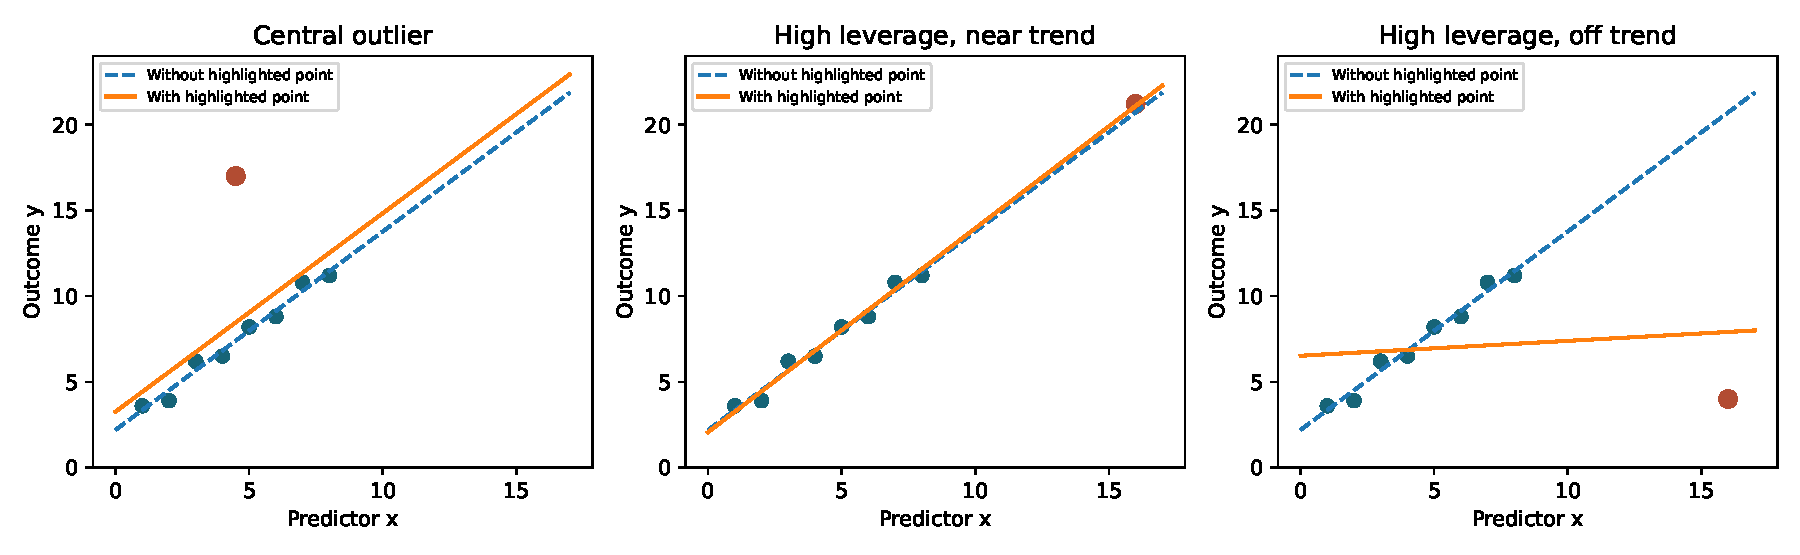
\includegraphics[width=\linewidth]{influence.pdf}\caption{Computed OLS fits for three illustrative configurations. The dashed line excludes the highlighted observation. Position in predictor space and change in the fitted line answer different questions.}\end{figure}
\section{Normal Q--Q plots: quantile, percentile, quartile}
A quantile is a distribution cutoff: $Q(p)=\inf\{y:F(y)\ge p\}$. The 90th percentile is $Q(0.90)$. Quartiles are $Q(0.25)$, $Q(0.50)$ and $Q(0.75)$. Q--Q means quantile--quantile, not quartile--quartile.
For a normal variable, $Q(p)=\mu+\sigma\Phi^{-1}(p)$. This linear relationship motivates comparing ordered observations $e_{(i)}$ with $z_i=\Phi^{-1}((i-0.5)/n)$; software plotting positions may differ slightly. The horizontal axis is typically theoretical normal quantiles and the vertical axis observed ordered residuals. A straight reference line need not be $y=x$.
Approximate linearity supports normal-like shape; systematic asymmetry suggests skewness. Relative to a suitable central line, heavy tails typically place the lower tail below and upper tail above it; light tails show the reverse. Finite-sample fluctuations, leverage and parameter estimation complicate interpretation. The plot does not establish independence, constant variance, correct mean structure or causality.
\begin{figure}[htbp]\centering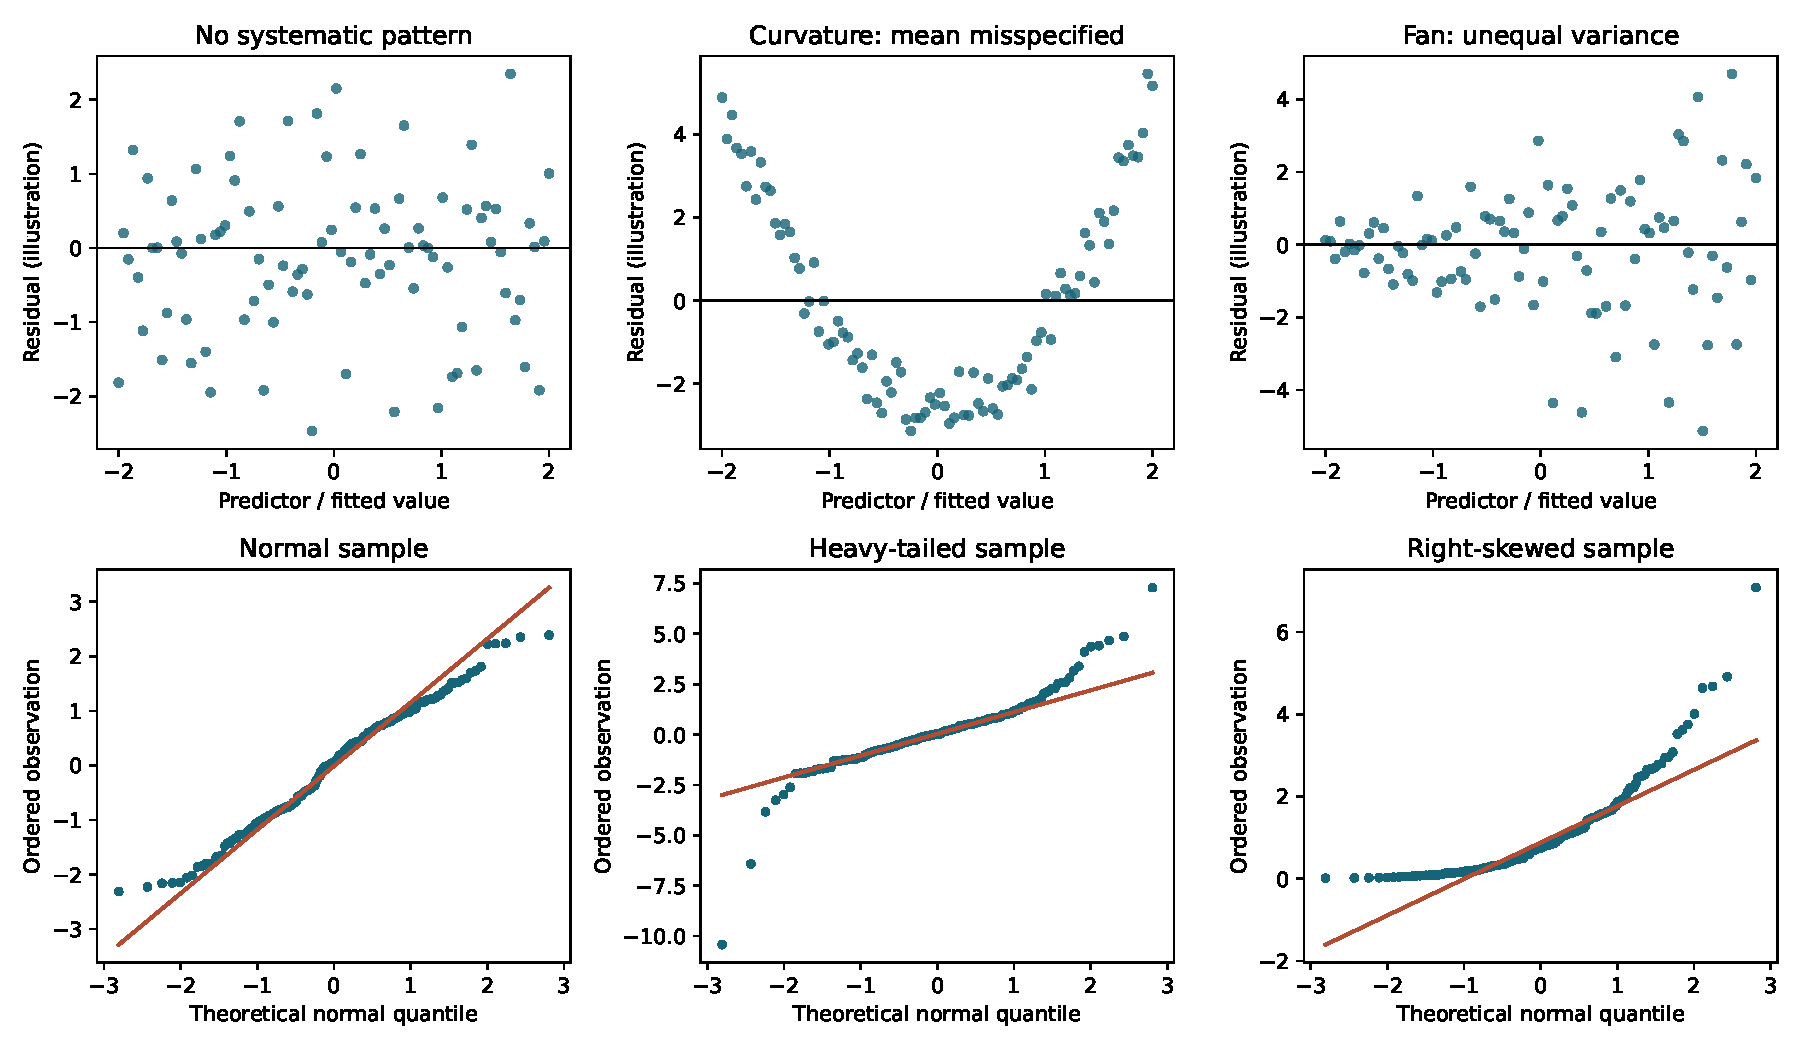
\includegraphics[width=\linewidth]{diagnostic-patterns.pdf}\caption{Simulated patterns, not empirical findings. Top: residual signatures to investigate. Bottom: Q--Q comparisons using independent simulated samples to isolate distribution shape; fitted regression residuals have additional dependence.}\end{figure}
\section{Why diagnostics require judgment}
The reference mathematics is precise; adequacy is purpose-dependent. Finite data cannot prove a model true. A formal test fixes an error-rate convention for specified alternatives, but small samples can miss important departures and large samples can detect negligible ones. Repeated testing and adapting the model to diagnostics can also distort subsequent inference.
Distinguish three statements: (1) a departure is detectable; (2) it changes the estimand's estimate or uncertainty; (3) it changes a scientific decision. Quantify the latter two through sensitivity analyses and validation. Report what was checked and what changed, rather than declaring that all assumptions were verified.
\section{Mathematical tests and their limits}
\subsection{Specified additional mean terms: partial F test}
Compare nested reduced and full models fitted to identical observations, with $q$ additional parameters and $p_F$ full-model parameters:
\[H_0:\beta_{\mathrm{added}}=0,\qquad F=\frac{(\mathrm{SSE}_R-\mathrm{SSE}_F)/q}{\mathrm{SSE}_F/(n-p_F)}.\]
Under a correct full mean model with independent normal, constant-variance errors, $F\sim F_{q,n-p_F}$ under $H_0$. For example, compare $y\sim x$ against $y\sim x+x^2$ to test a specified curvature term. Rejection supports the added terms; nonrejection does not prove linearity. RESET adds powers of fitted values as an omnibus specification screen and cannot identify the correct replacement model. Use robust Wald inference when justified if the classical covariance model fails.
\subsection{Breusch--Pagan / Koenker variance tests}
The null is constant conditional error variance. An auxiliary regression relates squared residuals to chosen variance predictors. In the usual studentized Koenker formulation, $LM=nR^2$ from this auxiliary regression is asymptotically $\chi_q^2$ under regularity and suitable moments; $q$ excludes its intercept. The original BP version uses a different normalization and stronger distributional assumptions. In R, \texttt{lmtest::bptest(fit)} defaults to the studentized version. Neither version detects every variance pattern. Mean misspecification can also produce apparent variance patterns.
\subsection{Serial dependence: Breusch--Godfrey}
For genuinely ordered data, regress residuals on original regressors and $q$ lagged residuals. Under regularity and a valid mean/dynamic specification, an LM statistic based on the effective auxiliary sample is asymptotically $\chi_q^2$ for the null of no serial correlation through those lags. Software differs in treatment of initial lags. Use \texttt{bgtest(fit, order=q)} only when ordering is meaningful. Serial tests are not substitutes for cluster-aware analysis.
\subsection{Normality and simulation calibration}
Shapiro--Wilk tests normality for an independent normal sample. Applying its usual reference distribution directly to fitted residuals ignores their design-dependent joint distribution. Treat an ordinary residual-based p-value cautiously. A parametric simulation can calibrate a residual statistic under the fitted normal linear model: simulate normal errors at fixed $X$, refit, recompute the same statistic, and compare with the observed value. This explicitly includes fitting and leverage in the reference distribution. It tests a specified normal-model reference, not all possible model errors.
\subsection{Assumptions needed for different conclusions}
OLS computation needs full column rank, not normality. Conditional unbiasedness needs the correct linear conditional mean and zero conditional error mean. Gauss--Markov efficiency additionally uses spherical covariance. Classical exact small-sample normal-theory inference uses normal errors. Suitable robust covariance estimators can address some covariance violations asymptotically; they do not repair confounding, a wrong mean, or unreliable data.
\section{A practical diagnostic workflow}
\begin{enumerate}
\item Define the target and design. Identify repeated measures, sampling weights, clusters, missingness and temporal order before choosing a model.
\item Check units, coding, impossible values and measurement processes. Preserve legitimate unusual observations.
\item Examine outcome/predictor distributions and scientifically plausible nonlinearities or interactions.
\item Fit a defensible initial model. Inspect residuals versus fitted values, each predictor and relevant time/group variables; inspect a Q--Q plot.
\item Quantify leverage, externally studentized residuals and influence. Investigate flagged cases and compare estimates with and without them as sensitivity analysis, not automatic exclusion.
\item Use targeted tests with stated hypotheses and assumptions. Avoid testing until all p-values exceed 0.05.
\item Compare scientifically justified alternatives. For prediction, use held-out or cross-validated evaluation with splits matching future deployment; keep tuning separate from final evaluation.
\item Report estimates, uncertainty, departures, sensitivity and remaining limitations.
\end{enumerate}
For clustered or survey data, ordinary $H$, Cook's distance and iid reference tests do not directly provide design-valid inference. Use the appropriate weighted/design model and cluster- or PSU-level sensitivity checks. For missing data, complete-case residuals describe the analyzed subset; they do not establish ignorability of missingness. For counts, binary outcomes or infection trajectories, choose appropriate likelihoods and dependence/observation models rather than forcing Gaussian diagnostics onto every outcome.
\section{Real-data R laboratory: industrial stack loss}
\textbf{Question:} How does mean stack loss vary with air flow, cooling-water temperature and acid concentration? The built-in \texttt{stackloss} dataset contains 21 observations from a nitric-acid plant. The response is an operational measure of ammonia loss; consult the dataset help for its scale and measurement details. This exercise estimates conditional associations, not causal effects. Allow about 45--60 minutes for the full lab, or 15 minutes for plots and influence only.
\lstinputlisting{diagnostics_practice.R}
\section{Practice with feedback}
\begin{enumerate}
\item A point lies far to the right but on the trend. Is it necessarily influential? \textit{Answer:} It has high leverage; actual influence requires sensitivity of fitted quantities. Check deletion.
\item A Q--Q plot is straight but the residual plot fans outward. Which assumption is questionable? \textit{Answer:} Constant conditional variance. A Q--Q plot alone cannot assess it.
\item If residuals sum to zero, is the conditional mean correctly specified? \textit{Answer:} No; this holds algebraically for OLS with an intercept.
\item A BP test gives $p=0.30$. Can you claim equal variances? \textit{Answer:} No; report insufficient evidence against the tested null and assess precision, power and graphics.
\item A coefficient changes sign after deleting one valid case. What next? \textit{Answer:} Report sensitivity, inspect coding and design, examine specification and data coverage; do not delete solely to obtain a desired conclusion.
\item Lab task: list the three largest Cook's distances, compare the full and deleted coefficient estimates, and explain whether the substantive conclusion changes. \textit{Feedback:} Rank cases from computed diagnostics; do not invent an influential case from a remembered textbook result. Compare changes on meaningful scales, with uncertainty.
\end{enumerate}
\section{Expert resources and a reading pathway}
This is a curated, broad pathway, not an exhaustive bibliography. Links were checked through source discovery on October 29, 2026. Package behavior can change; inspect installed help and session information.
\begin{enumerate}
\item \textbf{Penn State STAT 501}: \href{https://online.stat.psu.edu/stat501/Lesson11}{Lesson 11: Influential Points}; \href{https://online.stat.psu.edu/stat501/Lesson04}{Lesson 4: Model Assumptions}. Start here for worked distinctions among outliers, leverage and influence.
\item \textbf{NIST/SEMATECH}: \href{https://www.itl.nist.gov/div898/software/dataplot/refman1/auxillar/regrdiag.htm}{Regression diagnostics reference}. Use for a broad catalogue of diagnostic ideas and applied checks.
\item \textbf{R Core documentation}: \href{https://stat.ethz.ch/R-manual/R-devel/library/stats/html/plot.lm.html}{plot.lm}; \href{https://stat.ethz.ch/R-manual/R-devel/library/stats/html/influence.measures.html}{influence.measures}. Read for exact definitions used by software.
\item \textbf{lmtest authors' documentation}: \href{https://search.r-project.org/CRAN/refmans/lmtest/help/bptest.html}{bptest}; \href{https://search.r-project.org/CRAN/refmans/lmtest/html/bgtest.html}{bgtest}; \href{https://search.r-project.org/CRAN/refmans/lmtest/help/resettest.html}{resettest}. Study hypotheses, defaults and reference distributions before using tests.
\item \textbf{Frank E. Harrell Jr.}: \href{https://hbiostat.org/rmsc/}{Regression Modeling Strategies course notes}. Continue here for specification, nonlinear effects, missing data, overfitting and validation, especially in biomedical work.
\item \textbf{R datasets documentation}: \href{https://stat.ethz.ch/R-manual/R-devel/library/datasets/html/stackloss.html}{Brownlee's Stack Loss Plant Data}. Read the primary software dataset record before interpreting the lab.
\end{enumerate}
\textbf{Suggested sequence:} definitions and figures; Penn State examples; execute the lab; consult R/lmtest references; then Harrell's broader modeling strategy. A defensible report connects the scientific target, evidence of departures, and sensitivity of conclusions.

\section{Research computation: stability, covariance and reproducibility}
\subsection{QR and SVD instead of explicitly inverting normal equations}
The inverse formula is useful for theory. In computation use a stable least-squares solver. For $X=QR$, with $Q^TQ=I_p$, solve $R\widehat\beta=Q^Ty$. Then $H=QQ^T$ and $h_{ii}=\sum_{k=1}^p Q_{ik}^2$; a full $n\times n$ matrix is unnecessary for leverage. For rank checks and near collinearity, inspect singular values $X=U\Sigma V^T$. For full rank, $\kappa_2(X)=s_{\max}/s_{\min}$ and $\kappa_2(X^TX)=\kappa_2(X)^2$. Scaling helps conditioning but cannot create information absent from the design. A small normal-equation residual alone cannot certify accurate coefficients in an ill-conditioned problem.
\subsection{Coefficient deletion identity}
For case design vector $x_i$ (a column) and full-rank deleted design, the Sherman--Morrison identity gives
\[\widehat\beta-\widehat\beta_{(i)}
=\frac{(X^TX)^{-1}x_i e_i}{1-h_{ii}}.\]
Multiplying by $X$ and using $\|X(X^TX)^{-1}x_i\|^2=h_{ii}$ produces Cook's formula. This derivation separates mathematical identity from a practical influence threshold.
\subsection{HC3 and generalized least squares}
For independent observations with potentially unequal variances, an HC3 covariance estimator is
\[\widehat V_{HC3}=(X^TX)^{-1}\left\{\sum_i x_ix_i^T\frac{e_i^2}{(1-h_{ii})^2}\right\}(X^TX)^{-1}.\]
Its usual inferential justification is asymptotic; it is not an exact small-sample replacement for all classical tests. Cluster dependence needs cluster-aware methods and sufficient independent clusters.
For $\operatorname{Var}(\varepsilon\mid X)=\sigma^2\Omega$ with known positive-definite $\Omega$, factor $\Omega=LL^T$ and whiten: $y^*=L^{-1}y$, $X^*=L^{-1}X$. OLS on the transformed data gives
\[\widehat\beta_{GLS}=(X^T\Omega^{-1}X)^{-1}X^T\Omega^{-1}y.\]
Use triangular solves rather than explicit inverses. Diagnostics should examine the transformed error structure and the scientific plausibility of $\Omega$. Estimating $\Omega$ introduces additional uncertainty; feasible GLS does not inherit every exact known-covariance result.
\subsection{Independent computational checks}
The accompanying \texttt{verify\_diagnostics.py} uses NumPy least-squares/QR and explicit case deletion to verify projection idempotence, residual orthogonality, $\sum h_{ii}=p$, Cook's formula and deleted residual identities. On the seeded synthetic example, maximum absolute discrepancies were $5.41\times10^{-15}$ for Cook's distance and $2.94\times10^{-15}$ for deleted residuals. These validate numerical identities on this example, not universal scientific adequacy. The R laboratory is supplied as reproducible source but was not executed in the authoring environment; run it in R and retain session information before reporting results.
A stronger software exercise uses NIST certified reference data across multiple difficulty levels. Compare matched quantities under the exact specified model, intercept convention and units. Agreement checks numerical computation; it does not establish the model's scientific validity.
\section{Industry and major research-group practice: a public-source pathway}
The following translates public resources into training exercises. It is not a claim of access to proprietary pharmaceutical SOPs or internal procedures, nor a regulatory certification. Actual requirements depend on the study, organization and applicable guidance.
\subsection{NIST: measurement, industrial modeling and numerical assurance}
NIST's Statistical Reference Datasets provide certified computational targets. Pair these with the industrial stack-loss lab: separate data quality, numerical accuracy, model adequacy and decision consequences. An R\&D handoff should include the measurement units, calibration/provenance, fitted model, uncertainty, influential operating conditions and limits of extrapolation. Suggested extension (45 minutes): reproduce a linear-regression StRD dataset using QR, verify coefficients and residual SD against the certified values, and document relative/absolute tolerances with explanations.
\subsection{FDA Office of Biostatistics and ICH: clinical-development reasoning}
The FDA's May 2023 covariate-adjustment guidance addresses randomized parallel-group trials and prognostic baseline covariates; its stated scope excludes several other settings, including observational confounding adjustment and longitudinal repeated-measures modeling. Use the document for its actual scope, not as a universal regression manual. ICH E9(R1) supplies an estimand and sensitivity-analysis framework.
Training exercise (60--90 minutes): simulate a two-arm randomized trial with a baseline outcome predictor. Define the population, treatment contrast, outcome, handling of intercurrent events and summary measure before fitting ANCOVA. Prespecify adjustment; compare conventional and justified robust uncertainty, inspect nonlinear baseline relationships and treatment interactions, and assess sensitivity for the same target. Report post-hoc analyses as such. A changed estimand is a different question, not automatically a sensitivity analysis for the original one.
\subsection{Vanderbilt / Frank Harrell: modeling strategy and clinical prediction}
Harrell's publicly available Regression Modeling Strategies material and reproducible-research guidance provide a broader framework: preserve predictor information, consider nonlinear effects, control model complexity, account for missingness and evaluate optimism. A useful diagnostic report connects those choices to performance and uncertainty rather than requiring every plot to look ideal. Exercise (60 minutes): compare prespecified linear and spline forms under resampling; put all adaptive selection inside the resampling loop and evaluate calibration as well as prediction error.
\subsection{WEHI / Bioconductor limma: high-dimensional biomedical R\&D}
The limma documentation, associated with the WEHI bioinformatics resource, illustrates linear modeling for gene-expression experiments and empirical-Bayes variance moderation. The voom method estimates a mean--variance relationship and uses precision weights for RNA-seq analysis. This is a concrete example of adapting the covariance model to measurement technology instead of relying on unweighted Gaussian diagnostics for raw counts.
Exercise (90 minutes or more, optional): use a documented public limma/voom worked example. Check sample metadata and batch structure, inspect sample-level quality and mean--variance trends, verify design rank and estimability, define contrasts and adjust for multiplicity. Do not select genes by unadjusted $p<0.05$ across thousands of tests. Follow the method's own diagnostics; single-outcome OLS residual rules do not transfer unchanged.
\subsection{What a reviewable R\&D diagnostic package contains}
\begin{enumerate}
\item A short scientific question and estimand, population and unit of analysis.
\item A data dictionary, versioned provenance, processing/missingness rules and design information.
\item A prespecified primary model and planned sensitivity checks, with later deviations logged.
\item Stable numerical fitting, rank/conditioning checks and independent checks for critical computations.
\item An evidence table: diagnostic finding, plausible explanation, action, effect on target estimate/uncertainty and remaining uncertainty.
\item Appropriate validation, with participant/site/time splits when those represent intended deployment; no leakage from preprocessing or model selection.
\item Versioned scripts, seeds, package/environment records and an executable report; an independent reviewer can reproduce key outputs.
\end{enumerate}
For an infection-burden thesis, extend this structure to the observation process, reporting delays, temporal dependence and stochastic simulation. A residual distribution check alone cannot validate a transmission mechanism or identify epidemiological parameters.
\section{Additional primary resources for R\&D}
\begin{enumerate}
\item \href{https://www.nist.gov/itl/sed/statistical-reference-datasets}{NIST Statistical Reference Datasets}: numerical benchmarks.
\item \href{https://www.fda.gov/regulatory-information/search-fda-guidance-documents/adjusting-covariates-randomized-clinical-trials-drugs-and-biological-products}{FDA: Adjusting for Covariates in Randomized Clinical Trials (May 2023)}: scope-specific clinical-development guidance.
\item \href{https://www.ema.europa.eu/en/scientific-guidelines/ich-e9-statistical-principles-clinical-trials}{EMA: ICH E9 and E9(R1)}: statistical principles, estimands and sensitivity analysis.
\item \href{https://hbiostat.org/rr/}{Harrell: Reproducible Research}: reproducible statistical collaboration.
\item \href{https://www.bioconductor.org/packages/release/bioc/html/limma}{Bioconductor limma}: current package documentation, user guide and linked primary methods papers. \href{https://bioinf.wehi.edu.au/limma/}{WEHI limma resource}.
\end{enumerate}
\textbf{Maintenance:} Recheck guidance status and installed software documentation before a new project. Retain this dated note as a versioned learning reference, and keep study-specific analysis decisions in the project's own analysis plan.

\end{document}
